\documentclass{beamer}

\usepackage{amsfonts,amsmath}

\title{Spectral Rigid Body Dynamics}
\author{Mikola Lysenko}

\begin{document}

\newcommand{\R}{\mathbb{R}}

\maketitle

\begin{frame}
\frametitle{Overview}
\end{frame}

\begin{frame}
\frametitle{Rigid Body Dynamics}
Limiting case of continuum dynamics where elastic modulus is infinite.

Pros:
\begin{itemize}
\item Pretty accurate at human scales
\item Good for materials which are stiff
\item Efficient kinematic constraints (good for mechanism design)
\end{itemize}

Cons:
\begin{itemize}
\item Inaccurate at extremely small or large scales
\item Bad for materials with low elastic modulus
\item Not always solvable (See: Painleve's paradox)
\end{itemize}

\end{frame}

\begin{frame}
\frametitle{Configuration Space of a Rigid Body}
Must be a Euclidean isometry

\begin{center}
\includegraphics[height=1.4in]{figures/rigid_body.png}
\end{center}

Identified with translation + rotation, (ie $SE(d) \cong SO(d) \ltimes \R^d$)

Tangent space is isomorphic to $\mathfrak{so}(d+1)$ ($d+1 \times d+1$ skewsymmetric matrix)

Motion of a rigid body given by a curve, $q(t)$, in $SE(d)$.
	$\dot{q}(t)$ is the tangent curve.
\end{frame}


\begin{frame}
\frametitle{Lagrangian Mechanics}
Turns physics into an optimization problem.

For each path, $q : \R \to SE(d)$, define a functional
\[ \mathcal{L}(q) = T(q) - U(q) \]
Where $T(q)$ is the total kinetic energy along $q$ and $U$ is the potential energy.

$\mathcal{L}$ measures the work done along $q$

\bf{Physical trajectories correspond to paths of minimal work.}

\end{frame}


\begin{frame}
\frametitle{Rigid Motions in 2D}
For the sake of concreteness, let $d = 2$

Elements of $SE(2)$ are $3 \times 3$ matrices, parameterized by $(\theta, x, y)$:
\[ (\theta, x, y) = \left ( \begin{array}{ccc}
\cos(\theta) & \sin(\theta) & x \\
-\sin(\theta) & \cos(\theta) & y \\
0 & 0 & 1 \\
\end{array} \right) \]


\end{frame}


\end{document}

